Verformung von Metallen und ihren Legierungen.
Ich kann nach ausreichend Training Metall \textbf{kaltverformen}. Warum will ich das machen? Neben Show-off kann ich dabei Werkstoffcharakteristika
wie Festigkeit und Bruchdehnung beeinflussen. Hierbei steigt ersteres, zweiteres sinkt allerdings. Das kann jemand sich
erschließen wenn jemand sich im Falle einer Biegung vorstellt, dass das Material an der Außenkante der Biegung bereits über
den Hook'schen Bereich hinaus beansprucht wurde. Sich in anderen Worten bereits im plastischen Bereich befindet und so
den Weg bis zur Bruchdehnung verkürzt. In extremen Fällen hilft hier Nachglühen. So können Spannungen im Material durch
Rekristallisation ausgeglichen werden.
Alternativ kann jemand das Material im geglühten Zustand Formen (der Schmitt hat sowas gemacht) - \textbf{Warmumformen} genannt.
Hier wird während des Formungsprozesses das Material konstant über der Rekristallisationstemperatur gehalten. Das macht
den Formungsprozess nicht nur weniger Kräftezerrend, es ist auch möglich die Gefügestruktur und damit Eigenschaften wie
Duktilität des Materials direkt zu beeinflussen.
Wir wurden gelehrt, dass der Zugversuch der Apex unter den Materialprüfungen ist da hier die wichtigsten Eigenschaften
abgedeckt werden. Das zu prüfende Material wird in eine genormte Form gebracht und in die Apperatur eingespannt. Anschließend
wird bei genormter Geschwindigkeit das Material auseinander gezogen und hierbei die auftretende Spannung im Material
(durch den bekannten Querschnitt des Materials und kontinuierliche Messung der erforderlichen Kraft) über die sich
ergebende relative Längenänderung oder Dehnung \(\varepsilon \) aufgetragen. Ein sich hierbei ergebendes Diagram zeigt
Abbildung \ref{fig:luedi}.
\begin{figure}[h]
    \centering
    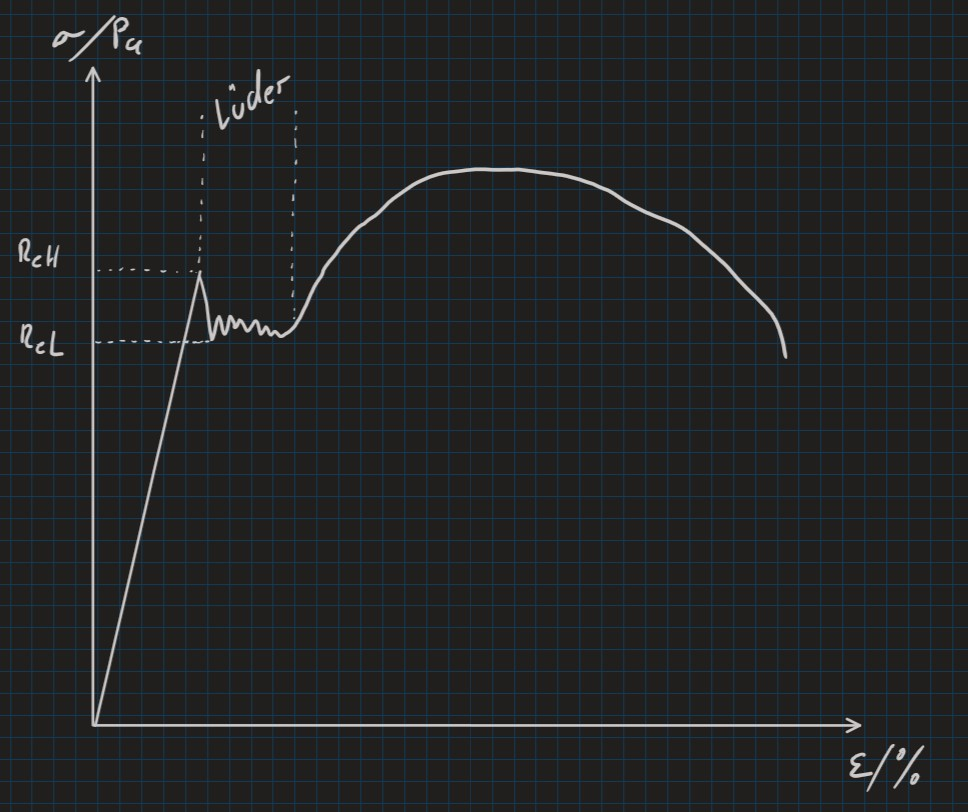
\includegraphics[width=0.5\textwidth]{entries/6/luedi.jpg}
    \caption{Skizze eines Zugdiagrams. Hook'scher Bereich bis Ende des linearen Teils.}
    \label{fig:luedi}
\end{figure}
Der sich seltsam verhaltende Teil wird durch eingelagerte Fremdatome im Material verursacht, die durch die Beanspruchung
aus ihren Plätzen zwischen den Gefügegrenzen vertrieben werden. Die Kennwerte \(R_{eH}\) und \(R_{eL}\) markieren hierbei
die obere (H) bzw. untere (L) Streckgrenze.
Habe ich es nun mit einem reinen Material zu tun (es gibt sicherlich auch Mischwerkstoffe mit ähnlichem Verhalten) fehlt
der Lüders-Teil wie in Abbildung \ref{fig:zug} skizziert und die Streckgrenzen sind nicht klar ersichtlich. Hier wird per
Konvention eine Linie parallel zur Hook'schen Geraden beginnend bei \(\varepsilon = 0.2\%\) eingezeichnet. Der Schnittpunkt
liefert hier die Spannung \(R_{p,0.2}\), bei der die Länge nach Entlastung \(0,2\%\cdot l_0\) beträgt. Erwähnenswert ist
hier noch da mir das bis dahin nicht so klar war, dass der E-Modul \(E\) gleich der Steigung im linearen Bereich ist 0o.
\begin{figure}[h]
    \centering
    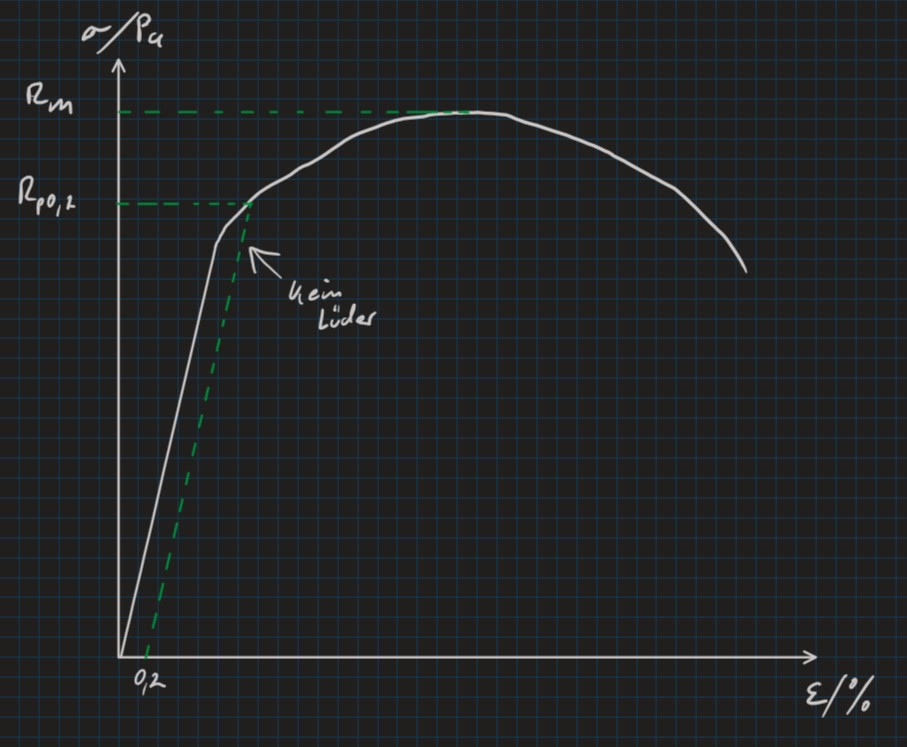
\includegraphics[width=0.5\textwidth]{entries/6/zug.jpg}
    \caption{Ungelüdertes Zugdiagram.}
    \label{fig:zug}
\end{figure}

Themenwechsel - quantitative Gefügeanalyse. Es ist unpraktikabel ein Material derart zu zerlegen bis jemand jedes einzelne
Korn frei gelegt hat um sie zu Vermessen und im Anschluss eine Aussage über ihre Volumenanteile im Urmaterial treffen zu
können. Statt dessen kann jemand sich etwas Statistik und Extrapolation zu Nutze machen. Ein Stück des zu prüfenden Materials
wird auf Glanz poliert und mikroskopisch mittels drei verschiedener Verfahren untersucht.
\newpage
\begin{figure}[h]
    \centering
    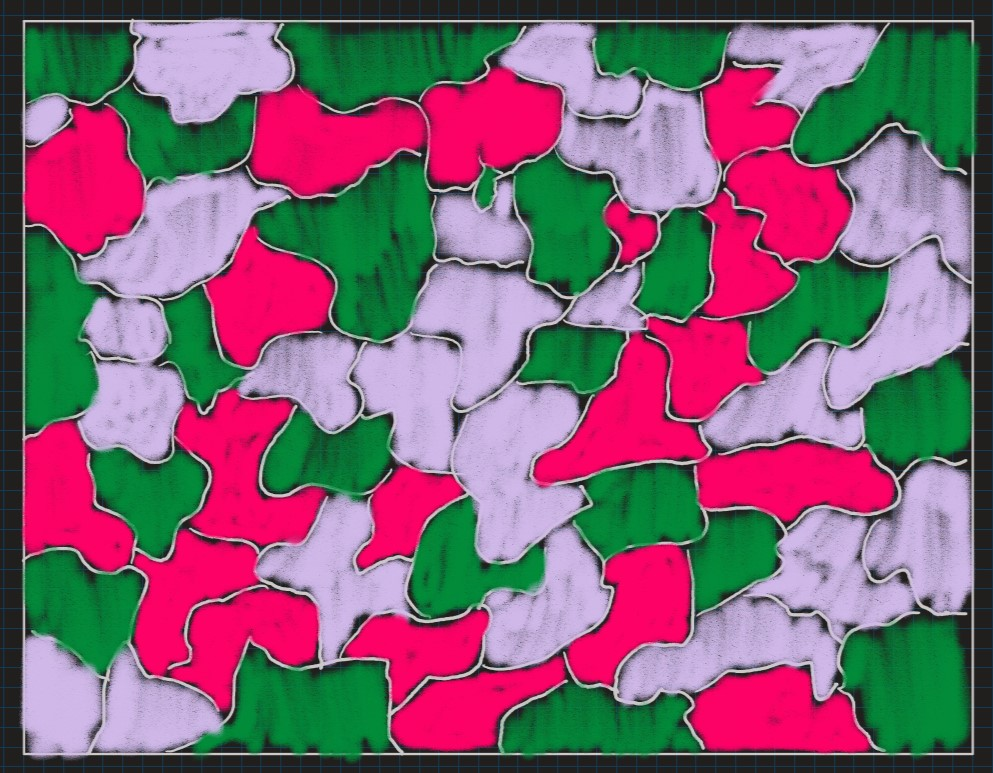
\includegraphics[width=0.5\textwidth]{entries/6/flaechen.jpg}
    \caption{Flächenanalyse}
    \label{fig:flaechen}
\end{figure}
\begin{enumerate}
    \item Körner Zählen -> \(N_{\alpha}, N_{\beta}, N_{\gamma}\).
    \item Gesamtfläche der Körner je Phase ermitteln -> \(A_{\alpha}, A_{\beta}, A_{\gamma}\).
    \item Volumenanteile \(v_{\alpha}, v_{\beta}, v_{\gamma}\) ergeben sich aus den jeweiligen Verhältnissen der Gesamtfläche zur Testfläche.
    \(v_{\alpha,\beta,\gamma} = \frac{A_{\alpha,\beta,\gamma}}{A_{\alpha,\beta,\gamma}}\).
\end{enumerate}

\begin{figure}[h]
    \centering
    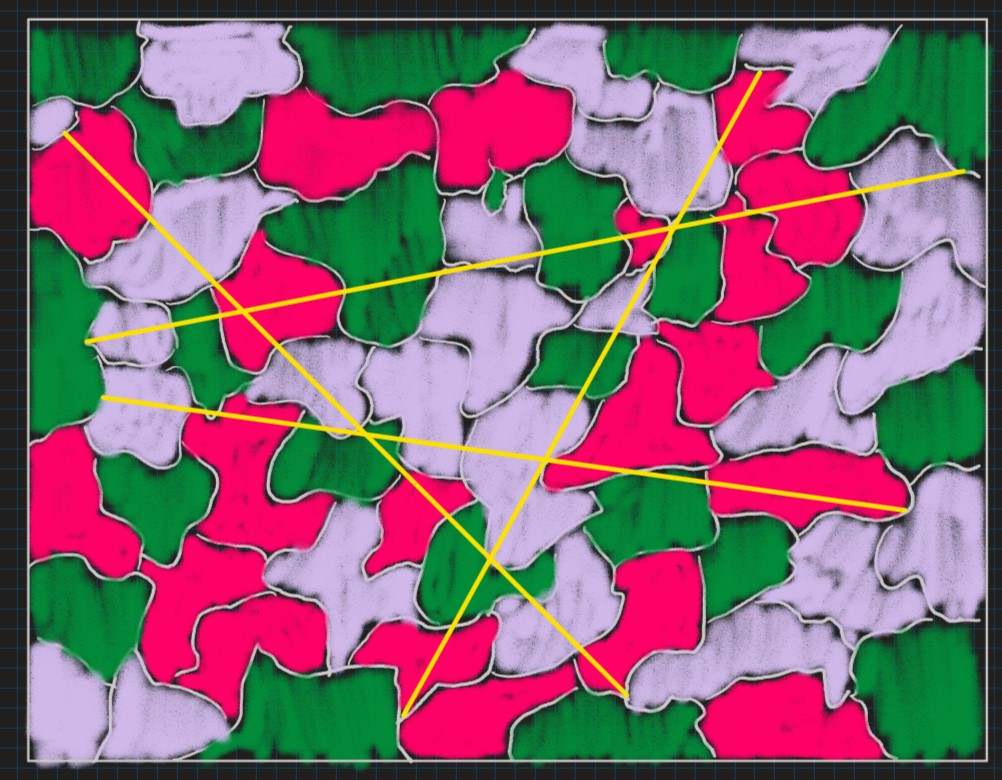
\includegraphics[width=0.5\textwidth]{entries/6/linien.jpg}
    \caption{Linienanalyse}
    \label{fig:flaechen}
\end{figure}
\begin{enumerate}
    \item Anzahl der Körner im Testschnitt zählen \(N_{\alpha T}, N_{\beta T}, N_{\gamma T}\).
    \item Beliebige Gerade durch die Schnittfläche
    ziehen beginnend und endend an Korngrenzen.
    \item Geschnittene Körner zählen -> \(N_{\alpha}, N_{\beta}, N_{\gamma}\).
    \item Ergebende Sehnenlängen der Schnitte messen
    \(L_{\alpha}, L_{\beta}, L_{\gamma}\).
    \item Schritte 2-4 \(n\) mal wiederholen.
    \item Der Quotient aus Summer aller Sehnenlängen einer Phase und Anzahl ihrer Körner im
    Testschnitt liefert die mittlere Korngröße. \( \overline{L_{\alpha,\beta\gamma}} = \frac{\sum_{k=1}^{n} ( \sum_{i=1}^{N_{\alpha}} L_{\alpha,i})}{ \sum_{k=1}^{n}N_{\alpha} } \).
    \item Volumenanteile ergeben sich als Verhältnis aus der Summe aller Sehnenlängen einer Sorte und der mittleren Korngröße
\end{enumerate}

\begin{figure}[h]
    \centering
    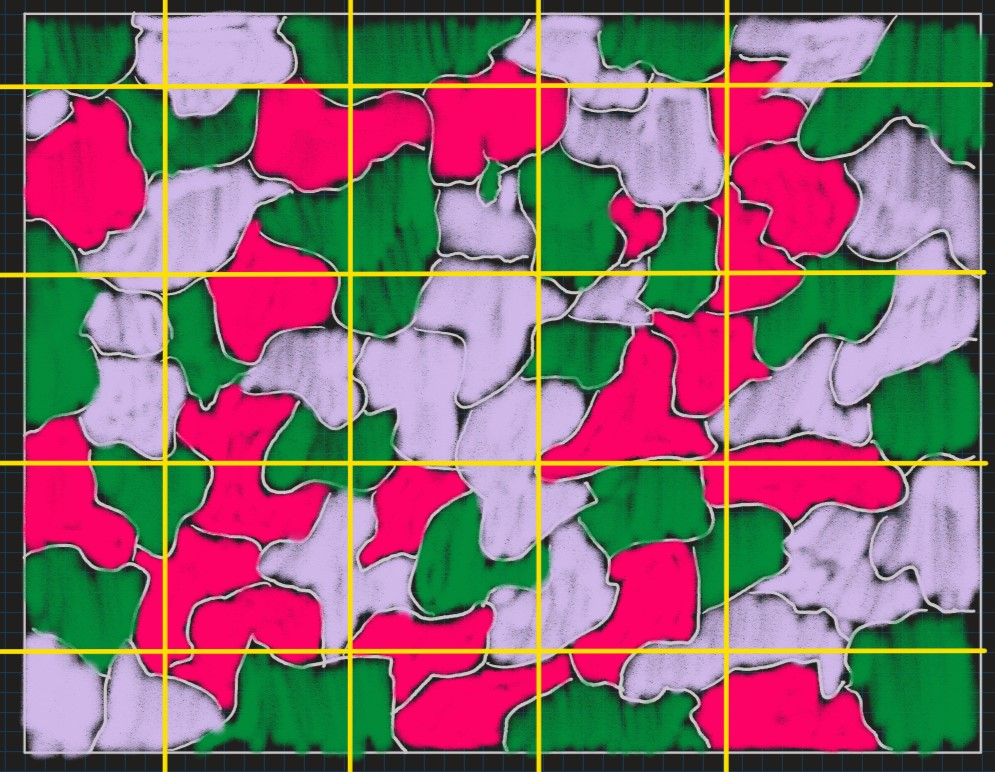
\includegraphics[width=0.5\textwidth]{entries/6/punkt.jpg}
    \caption{Punktanalyse}
    \label{fig:punkt}
\end{figure}
\begin{enumerate}
    \item Alle Körner im Testschnitt zählen -> \(N_T\).
    \item Gleichmäßiges Raster über den Testschnitt legen.
    \item Körner zählen, die von einem der Rasterkreuze getroffen werden -> \(N_{\alpha T}, N_{\beta T}, N_{\gamma T}\).
    \item Volumenanteil ergibt sich als Quotient aus Anzahl der getroffenen Körner und Gesamtzahl aller Körner im Testschnitt.
\end{enumerate}
